\section*{电磁感应}

\subsubsection*{一. 选择题}

2. 如图所示,矩形区域为均匀恒稳磁场,半圆形闭合导线回路在纸面内绕轴$O$作逆时针方向匀角速转动,$O$点时圆心且恰好落在磁场的边缘上,半圆形闭合导线完全在磁场外时开始计时,图中的$\varepsilon$-$t$函数图像中哪一条属于半圆形导线回路中产生的感应电动势.\fbox{(A)}.

图2.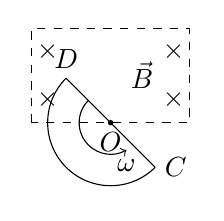
\begin{tikzpicture}
\draw[dashed] (-1,0) rectangle (1,1.2);
\draw (-0.8, 0.3) node {$\times$};
\draw (-0.8, 0.9) node {$\times$};
\draw (0.8, 0.3) node {$\times$};
\draw (0.8, 0.9) node {$\times$};
\draw (0.4, 0.6) node {$\vec B$};
\fill (0,0) node[below] {$O$} circle (1pt);
\draw (135:0.8) node[above] {$D$} -- (315:0.8) node[right] {$C$};
\draw (315:0.8) arc (315:135:0.8);
\draw[->] (135:0.4) arc (135:300:0.4) node[below] {$\omega$};
\end{tikzpicture}
(A)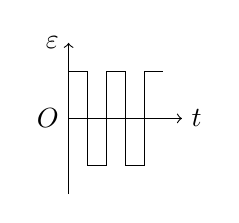
\begin{tikzpicture}[scale=1.2]
\draw[->] (0,0) node[left] {$O$} -- (1.2,0) node[right] {$t$};
\draw[->] (0,-0.8) -- (0,0.8) node[left] {$\varepsilon$};
\draw (0,0.5) -- (0.2,0.5) -- (0.2,-0.5) -- (0.4,-0.5) -- (0.4,0.5) -- (0.6,0.5) -- (0.6,-0.5) -- (0.8,-0.5) -- (0.8,0.5) -- (1,0.5);
\end{tikzpicture}
图3.\begin{tikzpicture}
% \draw[help lines] (0,-2) grid (6,0);
\draw[dashed] (0,0) -- (6,0);
\draw[->] (1,0) -- (3,0) node[above] {$I$};
\draw (3,0) -- (5,0);
\foreach \x in {0, 1.5, 3, 4.5}
    \draw (\x,-1) rectangle +(1,0.5);
\draw[dashdotted] (0.5,-1.5) -- (0.5,-0.2);
\draw[->] (0.4,-1.1) parabola[bend at end] (0.7,-1.3) node[right] {$\omega$};
\draw (0.5,-1.9) node {(1)};
\draw[dashdotted] (1.2,-0.75) -- (2.8,-0.75);
\draw[->] (2.7,-0.5) parabola[bend at end] (2.6,-0.9) node[right] {$\omega$};
\draw (2,-1.9) node {(2)};
\draw[->] (3.5,-1.1) -- (3.5,-1.6) node[right] {$\vec v$};
\draw (3.5,-1.9) node {(3)};
\draw (4.7,-0.75) node {$\times$} circle(0.5em);
\draw (5,-0.75) node {$\vec v$};
\draw (5,-1.2) node {\small 向纸面平移};
\draw (5,-1.9) node {(4)};
\end{tikzpicture}

3. 如图所示,一矩形线圈,放在一无限长载流直导线附近,开始时线圈与导线在同一平面内,矩形的长边与导线平行.若矩形线圈以图中所示四种方式运动,则在开始瞬间,以图\fbox{(3)}方式运动的矩形线圈中的感应电流最大.

4. 如图,长度为$l$的直导线$ab$在均匀磁场$\vec B$中以速度$\vec v$移动,直导线$ab$中的电动势为\fbox{0}.

5. 一根长度为$L$的铜棒,在均匀磁场$\vec B$中以匀角速度$\omega$绕通过其一端$O$的定轴旋转着,$\vec B$的方向垂直铜棒转动的平面,如图所示.设$t=0$时,铜棒与$Ob$成$\theta$角($b$为铜棒转动的平面上的一个固定点),则在任意时刻$t$这根铜棒两端之间的感应电动势是\fbox{$\frac{1}{2}\omega L^2B$}.

6. 如图所示,导体棒$AB$在均匀磁场$\vec B$中绕通过$C$点的垂直与棒长且沿磁场方向的轴$OO'$转动(角速度$\vec\omega$与$\vec B$同方向),$BC$的长度为棒长的$1/3$,则\fbox{$A$点比$B$点电势高}.

8. 尺寸相同的铁环与铜环所包围的面积中,通以相同变化率的磁通量,当不计环的自感时,环中\ul{感应电动势相同,感应电流不同}.

9. 自感为0.25H的线圈中,当电流在(1/16)s内由2A均匀减小到零时,线圈中自感电动势的大小为\fbox{8.0V}.

10. 两个通有电流的平面圆线圈相距不远,如果要使其互感系数近似为零,则应调整线圈的取向使得\ul{一个线圈平面平行于两圆心连线,另一个线圈平面垂直于两圆心连线}.

\subsubsection*{二. 填空题}

36. 一导线被弯成如图所示形状,$acb$为半径为$R$的四分之三圆弧,直线段$Oa$长为$R$.若此导线放在匀强磁场$\vec B$中,$\vec B$的方向垂直纸面向内.导线以角速度$\omega$在图面内绕$O$点匀速转动,则此导线中的动生电动势\fbox{$\varepsilon_i=\frac{5}{2}B\omega R^2$},电势最高点是\fbox{$O$点}.

41. 一自感线圈中,电流强度在0.002s内均匀地由10A增加到12A,此过程中线圈内自感电动势为400V,则线圈的自感系数\fbox{$L=0.400$H}.

42. 有两个长度相同,匝数相同,截面积不同的长直螺线管,通以相同大小的电流.现将小螺线管完全放入大螺线管里(两者轴线重合),且使两者产生的磁场方向一致,则小螺线管内的磁能密度是原来的\fbox{4倍};若使两线管产生的磁场方向相反,则小螺线管中的磁能密度为\fbox{0}(忽略边缘效应).

43. 自感系数$L=0.3$H的螺线管中通以$I=8$A的电流时,螺线管存储的磁场能量\fbox{$W=9.6$J}.

44. 真空中两只长直螺线管1和2,长度相等,单层密绕匝数相同,直径之比$d_1:d_2=1:4$.当它们通以相同电流时,两螺线管贮存的磁能之比为\fbox{$W_1:W_2=1:16$}.

\subsubsection*{三. 计算题}

50. 无限长直导线,通以常定电流$I$.有一与之共面的直角三角形线圈$ABC$.已知$AC$边长为$b$,且与长直导线平行,$BC$边长为$a$.若线圈以垂直于导线方向的速度$\vec v$向右平移,当$B$点与长直导线的距离为$d$时,求线圈$ABC$内的感应电动势的大小和方向.
\SL{取顺时针绕向为正,穿过小阴影面积的元磁通量
$\d\varPhi=\frac{\mu_0I}{2\pi(r+x)}\cdot\frac{b}{a}x\d x$,\pp
式中$r$是$t$时刻$B$点与长直导线的距离.\\
总磁通量
$\varPhi=\frac{\mu_0Ib}{2\pi a}\int_0^a\frac{x}{r+x}\d x=\frac{\mu_0Ib}{2\pi a}(a-r\ln\frac{a+r}{r})$.\\
感应电动势的大小
$\varepsilon_i=-\frac{\d\varPhi}{\d t}=\frac{\mu_0Ib}{2\pi a}(\ln\frac{a+r}{r}-\frac{a}{a+r})\frac{\d r}{\d t}$,\pp
当$r=d$时,
$\varepsilon_i=\frac{\mu_0Ib}{2\pi a}(\ln\frac{a+d}{d}-\frac{a}{a+d})v$,
顺时针方向.
}
51. 如图所示,长直导线$AB$中的电流$I$沿导线向上,并以$\d I/\d t=2$A/s的变化率均匀增长.导线附近放一个与之同面的直角三角形线框,其一边与导线平行,距离为5cm.线框宽10cm,高20cm,求此线框中产生的感应电动势的大小和方向.
\SL{取顺时针绕向为正,元磁通量
$\d\varPhi=\frac{\mu_0I}{2\pi(0.05+x)}\cdot\frac{0.20}{0.10}(0.10-x)\d x$.\\
穿过直角三角形线框所围面积的总磁通量\pp
$\varPhi=\frac{\mu_0I}{2\pi}\int_0^{0.10}\frac{-2x+0.20}{x+0.05}\d x=-\frac{\mu_0Ib}{\pi}+\frac{0.15\mu_0I}{\pi}\ln3$.\\
三角形线框中的感应电动势大小为\pp
$\varepsilon_i=-\frac{\d\varPhi}{\d t}=-\frac{0.15\mu_0}{\pi}\ln3\frac{\d I}{\d t}=-5.18\E{-8}$V,
逆时针方向.
}
53. 如图所示,两条平行长直导线和一个矩形导线框共面,且导线框的一个边与长直导线平行,它到两长直导线的距离分别为$r_1$,$r_2$.已知两导线中电流都为$I=I_0\sin\omega t$,其中$I_0$和$\omega$为常数,$t$为时间.导线框长为$a$宽为$b$,求导线框中的感应电动势.
\SL{两个载同向电流的长直导线在坐标$x$处所产生的磁场为
$B=\frac{\mu_0}{\pi}(\frac1x+\frac1{x-r_1+r_2})$.\\
取顺时针绕向为正,则
$\varPhi=\int B\d S=\frac{\mu_0Ia}{2\pi}(\int_i^{i+b}\frac{\d x}{x}+\int_i^{i+b}\frac{\d x}{x-r_1+r_2})
=\frac{\mu_0Ia}{2\pi}\ln(\frac{r_1+b}{r_1}\cdot\frac{r_2+b}{r_2})$.\\
所以
$\varepsilon_i=-\frac{\d\varPhi}{\d t}
=-\frac{\mu_0a}{2\pi}\ln[\frac{(r_1+b)(r_2+b)}{r_1r_2}]\frac{\d I}{\d t}
=-\frac{\mu_0I_0a\omega}{2\pi}\ln[\frac{(r_1+b)(r_2+b)}{r_1r_2}]\cos\omega t$.
}
56. 如图所示,一长直导线中通有电流$I$,有一垂直于导线长度为$l$的金属棒$AB$在包含导线的平面内,以恒定的速度$\vec v$沿与棒成$\theta$角的方向移动.开始时,棒的$A$端到导线的距离为$a$,求任意时刻金属棒中的动生电动势,并指出棒哪端的电势高.
\SL{$v_\perp=v\sin\theta$, $v_\parallel=v\cos\theta$,\\
$\varepsilon_i=\int\dh\varepsilon_i=-\int_{a+vt\cos\theta}^{a+l+vt\cos\theta}\frac{\mu_0I}{2\pi x}v\sin\theta\d x$
($\varepsilon_i$以$A\to B$为正).\\
$\varepsilon_i=-\frac{\mu_0I}{2\pi}v\sin\theta\ln\frac{a+l+vt\cos\theta}{a+vt\cos\theta}$,
$A$端的电势高.
}
57. 
\SL{
}
58. 
\SL{
}




















